\documentclass[12pt,letterpaper]{article}
\usepackage[margin=1in]{geometry}
\usepackage{fancyhdr}
\usepackage[utf8]{inputenc}
\usepackage{palatino}
\usepackage{microtype}
\usepackage{hyperref}
\usepackage{graphicx}
\usepackage{lastpage}
\usepackage[hang,small]{caption}
\usepackage{titlesec}
\usepackage{amsmath,amssymb}
\usepackage{multirow}

\renewcommand{\headrulewidth}{0pt}
\fancyfoot{}
\fancyfoot[C]{\sf Page \thepage\ of \pageref{LastPage}}
\pagestyle{fancy}

\titleformat{\section}{\bfseries\Large}{\arabic{\thesection}}{1em}{}
\titleformat{\subsection}{\bfseries\large}{\arabic{\thesection}.\arabic{\thesubsection}}{1em}{}
\titleformat{\subsubsection}{\itshape}{\arabic{\thesection}.\arabic{\thesubsection}.\arabic{\thesubsubsection}}{1em}{}

\setlength{\parindent}{0cm}
\setlength{\parskip}{0.8em}

\captionsetup[figure]{labelfont=it,font=it}
\captionsetup[table]{labelfont={it,sc},font={it,sc}}

\hypersetup{colorlinks,
  linkcolor = black,
  citecolor = black,
  urlcolor  = black}
\urlstyle{same}



\begin{document}

Soo-Hyun Yoo \\
ST314 \\
Data Analysis 4 \\
November 11, 2014

\begin{enumerate}
  \item
    \begin{enumerate}
      \item \hfill\\
        \begin{table}[!h]
          \centering
          \begin{tabular}{|c|c|c|c|} \hline
                 & Mean & Std. Dev. & Sample size \\ \hline
            US   & 21.48127 & 5.163967 & 347 \\ \hline
            Intl & 23.83743 & 5.820344 & 732 \\ \hline
          \end{tabular}
        \end{table}

      \item \hfill\\ 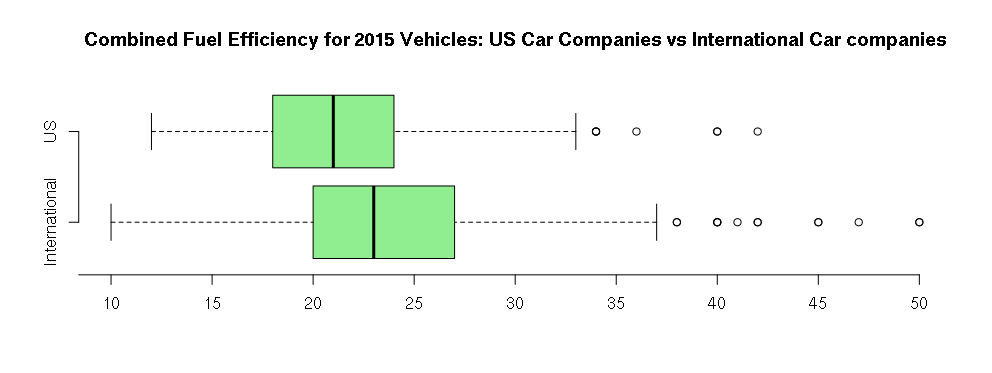
\includegraphics[width=0.8\textwidth]{1b.png}

        Both US and International mpg figures appear evenly distributed with
        a few outliers to the right, but the International fuel efficiency is
        clearly greater than the US fuel efficiency based on both IQRs as well
        as the median.

      \item $H_0: \mu_1 - \mu_2 = 0$

        $H_a: \mu_1 - \mu_2 \ne 0$

      \item $t = \cfrac{\bar{X_1} - \bar{X_2} - \Delta_0}{\sqrt{\frac{s_1^2}{n}+\frac{s_2^2}{n}}} = \cfrac{21.481-23.837}{\sqrt{\frac{5.164^2}{347}+\frac{5.820^2}{732}}} = \boxed{-6.714}$

      \item Satterwaite approximation for $v = 347 - 1 = \boxed{346}$

        p-value is $cdf(-6.714, 346) = \boxed{0.000}$

      \item $CI = (\bar{X_1} - \bar{X_2}) \pm t_{0.05,346}\sqrt{\frac{s_1^2}{n_1}+\frac{s_2^2}{n_2}} = (21.481-23.837) \pm 1.6493\sqrt{\frac{5.164^2}{347}+\frac{5.820^2}{732}} = \boxed{(-2.935, -1.777)}$

      \item R gives $t = 6.7147$, $v = 758.081$, p-value $= 3.696e-11$, and
        a confidence interval of $(1.778, 2.934)$. The $t$, $v$, and p-values
        are slightly different from the hand calculations, probably due to
        rounding errors. The confidence interval is simply negated from the
        hand calculations due to different ordering of $\mu_1$ and $\mu_2$.

      \item There is convincing evidence of a difference between the average
        fuel efficiency of cars made by US companies and those made by
        international companies. We reject the null hypothesis at the 0.05
        significance level with a two-sided p-value of $0.000$ from
        a two-sample t test with 758 degrees of freedom. The estimated
        difference in average fuel efficiency is 2.356 with a 90\% confidence
        interval of 1.778 to 2.934. That is on average, there is definitely
        a difference in fuel efficiency between cars made by US companies and
        those made by international companies.

      \item
        \begin{verbatim}
# Summary Statistics
USMean = mean(CombFE[US=="US"])
USMean
USStdDev = sd(CombFE[US=="US"])
USStdDev 
USsamplesize = length(CombFE[US=="US"])
USsamplesize
INTMean = mean(CombFE[US=="International"])
INTMean
INTStdDev = sd(CombFE[US=="International"])
INTStdDev 
INTsamplesize = length(CombFE[US=="International"])
INTsamplesize

# Box Plot
boxplot(CombFE~US, data = mpg2015fefsub,
        horizontal = TRUE, col= "light green",
        main = "Combined Fuel Efficiency for 2015
        Vehicles: US Car Companies vs International
        Car companies", axes = FALSE)
axis(1, seq(0,50, 5))
axis(2, 1:2, labels= c("International", "US"), las=0,
     cex.axis= 1)

# Two Sample T Test
t.test(CombFE~US)
          \end{verbatim}
        \end{enumerate}

  \item
    \begin{enumerate}
      \item \hfill\\ 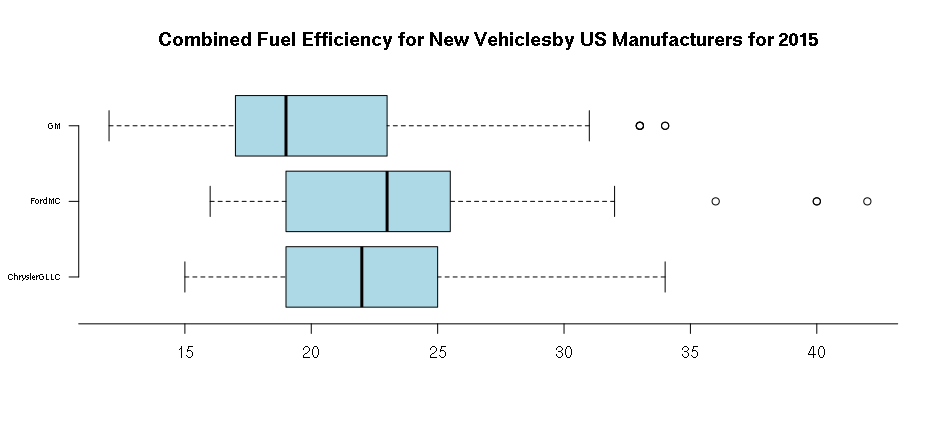
\includegraphics[width=0.8\textwidth]{2a.png}

        There is definitely a difference between differen US manufacturers.
        Ford's median fuel efficiency, for example, is nearly coincident with
        GM's 3rd IQR.

      \item $H_0: \mu_1 = \mu_2 = \mu_3$

        $H_a: \mu_1 \ne \mu_2 \ne \mu_3$

      \item R output:
        \begin{verbatim}
> mod = aov(CombFE~MfrName, data =onlyUS)
> summary(mod)

             Df Sum Sq Mean Sq F value   Pr(>F)    
MfrName       2    472  236.14   9.279 0.000119 ***
Residuals   344   8754   25.45                     
---
Signif. codes:  0 ‘***’ 0.001 ‘**’ 0.01 ‘*’ 0.05 ‘.’ 0.1 ‘ ’ 1
        \end{verbatim}

      \item R output:
        \begin{verbatim}
> TukeyHSD(mod, conf.level = 0.95)

Tukey multiple comparisons of means
95% family-wise confidence level

Fit: aov(formula = CombFE ~ MfrName, data = onlyUS)

$MfrName
                         diff        lwr        upr     p adj
FordMC-ChryslerGLLC  1.273016 -0.6193757  3.1654075 0.2541443
GM-ChryslerGLLC     -1.693642 -3.1533274 -0.2339564 0.0181726
GM-FordMC           -2.966658 -4.7061889 -1.2271267 0.0002156
        \end{verbatim}
    \end{enumerate}
\end{enumerate}

\end{document}

